\documentclass[11pt,twoside, authoryear]{elsarticle}
\usepackage[frenchb, english]{babel}
\usepackage[utf8]{inputenc}
%\usepackage[utf8]{fontenc}
%\usepackage[ansinew]{inputenc}
\usepackage{setspace}
\usepackage{babel,varioref}
\usepackage{supertabular}
\usepackage{graphicx}
%\usepackage[pdftex]{graphicx}
%\DeclareGraphicsExtensions{.pdf,.mps,.png,.jpg,.eps}
\usepackage{lscape}
\usepackage[authoryear]{natbib}
%\usepackage[frenchb,english]{babel}
\usepackage{multirow}
\usepackage{ifthen}
%\usepackage{harvard}
\usepackage{vmargin}
\usepackage{verbatim}
\usepackage{array}
%\usepackage[authoryear]{natbib}
\usepackage{hyperref}
\hypersetup{colorlinks=true,linkcolor=Black, citecolor=blue, urlcolor=blue}
%\setmarginsrb{2cm}{2cm}{2cm}{2cm}{0cm}{0cm}{0cm}{0cm}
\usepackage{booktabs,caption,fixltx2e}

\usepackage[flushleft]{threeparttable}
\makeatletter
\def\ps@pprintTitle{%
  \let\@oddhead\@empty
  \let\@evenhead\@empty
  \let\@oddfoot\@empty
  \let\@evenfoot\@oddfoot
}
\makeatother
\usepackage{adjustbox}
\usepackage{chngcntr}
\counterwithin{table}{section}
%\usepackage[round]{natbib}

\renewcommand{\thesection}{\Alph{section}}

% \newcommand\section[1]{%
%   \refstepcounter{section}%
%   \addcontentsline{toc}{section}{\protect\numberline{\thesection}#1}%
%   \sectionmark{#1}}
%   }


% % \refstepcounter{section}%
% %   \addcontentsline{toc}{section}{\protect\numberline{\thesection}#1}%
% %   \sectionmark{#1}}



%   \newcommand\subsection[1]{%
%   \refstepcounter{subsection}%
%   \addcontentsline{toc}{subsection}{\protect\numberline{\thesubsection}#1}%
%   %\subsectionmark{#1}
%   }

%\EnableSectionsInLOFT



\begin{document}
\title{\textbf{Beyond the Iceberg Hypothesis: \\Opening the Black Box of Transport Costs}\\Online Appendix (Not for publication)}

\urlstyle{rm}
\author{Guillaume Daudin\footnote{\noindent Corresponding author. Universit\'{e} Paris-Dauphine, PSL Research University, LEDa-DIAL, UMR 225, France \&
SciencesPo, Observatoire Français des Conjonctures \'{E}conomiques (OFCE), France; email: \url{guillaume.daudin@dauphine.fr}} \qquad \quad Jérôme Héricourt\footnote{\noindent Corresponding author. Université de Lille - LEM-CNRS (UMR 9221) and CEPII; email: \url{jerome.hericourt@univ-lille1.fr}} \qquad \quad Lise Patureau\footnote{\noindent Universit\'{e} Paris-Dauphine, PSL Research University, LEDa, France ; email: \url{lise.patureau@dauphine.fr}}}
%\date{\vspace{-5ex}}

%Modèle additif seul
%+ableaux avec toutes les années en 3 digit et en 4 digit. Harmoniser la présentation des résultats (cf table 1 du papier)
%es résultats sur la version Hummels mais avec sa pondération: en annexe du papier? En online appendix?


\maketitle





%\newpage

\tableofcontents
\vspace{1cm}
\newpage
\listoftables

\newpage
%\section{\label{sec:addi}Additional Tables}


	\renewcommand\thesubsubsection{\Alph{subsection}.\arabic{subsubsection}}
	
	\renewcommand\thesubsection{\Alph{subsection}}
	
	
\subsection{Additive-costs only Model \label{secoa:additive_only}}

%%%% RAW TABLE TO BE FOUND AT: "...\Dropbox\Papier_Lise_Guillaume\trade_cost\results\3_models"
% modele iceberg tout seul : terme nlI
% colonnes L à U: modèle avec les deux
% termes nla, de V à Z, modèles avec que de l'additif
%nlI quer iceberg
%nla que additif
%nl : les deux
\setcounter{table}{0}
\renewcommand{\thetable}{A.\arabic{table}}
%\subsubsection{Nominal Exchange Rate Volatility}


\begin{table}[htbp]
  \centering
  \footnotesize{
  \caption{Transport costs estimates: Summary \label{sec_oa:add_only}}
  \begin{center}
    \begin{tabular}{l|cc|cc}
      \hline \hline
    \multicolumn{5}{c}{Mean value over 1974-2013}   \\
    \# digit & \multicolumn{2}{c}{3 digits} & \multicolumn{2}{c}{4 digits ($^\ast$)} \\ \hline
    Mode  & Vessel & Air ($^{\ast \ast}$) & Vessel & Air \\ \hline
    \multicolumn{5}{l}{\textbf{With only Additive Transport Costs} ($\widehat{t}^{add}$, in \%)}  \\ \hline
    Mean  & 9.2 & 5.1 & 8.0 & 5.8 \\
    Median & 5.7 & 2.4 & 5.5 & 2.5 \\ \hline

       \multicolumn{5}{l}{\textbf{Data} ($p/\widetilde{p}$, in \%) } \\ \hline
        Mean & 5.3 & 5.0& 5.6&3.9 \\
        Median & 4.3 & 2.0 & 4.4& 1.9 \\ \hline
        \# obs. & 29279 & 28207 & 29317 & 27680 \\
    \# origin country & 188 & 191 & 188 & 189 \\
    \# products & 230 & 211 & 666 & 567 \\  \hline \hline
  \end{tabular}
    \end{center}}
\parbox[l]{10cm}{\tiny{Notes: Statistics are obtained weighting each observation by its value relative to total trade flows. The additive term is expressed in fraction of fas price. ($^\ast$): Four 4-digit estimation: 0n selected years. ($^{\ast \ast}$): 1989 omitted in 3-digit estimation for air.}}
\end{table}%







%
%XXXXXX
%
%
%			SECTION 2 / ALTERNATIVE MEASURES OF FIRM PERFORMANCE
%			
%			
%					
%XXXXXX
%
%
%
%\subsection{At a more disaggregated level}


\textbf{A mon avis, a mettre en online appendix. Expliquer comment se fait la decomposition en secteurs primaire/manuf.}

In this Section, we characterize the time trend in international transport costs at a more disaggregated level, by distinguishing the trade flows for primary goods and manufactured goods. The evolution in transport costs over time, by transport mode (overall transport costs and composition effects excluded) are reported in \ref{fig:totalTC_compeffects_excl_manuf} for the manufacturing sector, and in Figure \ref{fig:totalTC_compeffects_excl_primary} for the primary goods.

\begin{figure}[htbp]
\caption{Transport costs (with and without composition effects), Manufacturing}
\label{fig:totalTC_compeffects_excl_manuf}
\begin{center}
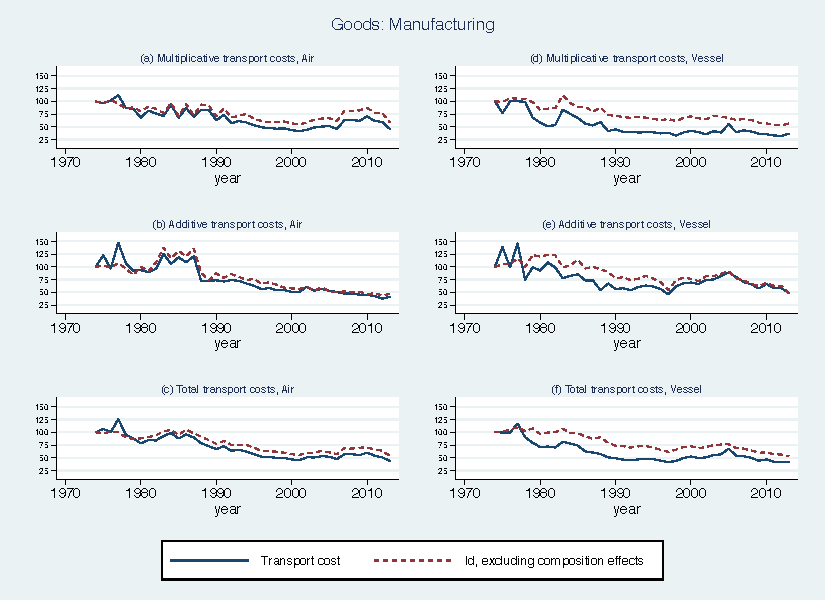
\includegraphics[height=4in]
{graph_composition_manuf.pdf}
\end{center}
\end{figure}

\begin{figure}[htbp]
\caption{Transport costs (with and without composition effects), Primary goods}
\label{fig:totalTC_compeffects_excl_primary}
\begin{center}
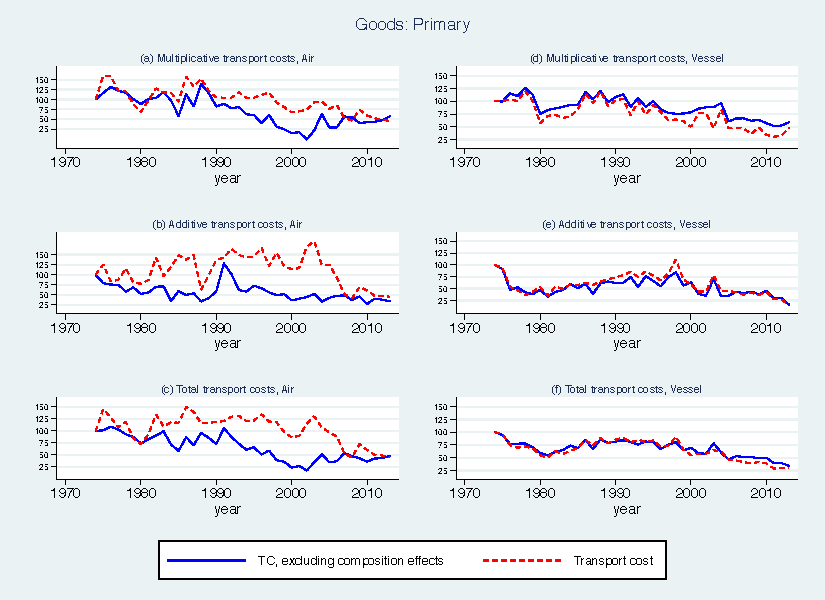
\includegraphics[height=4in]
{graph_composition_primary.pdf}
\end{center}
\end{figure}



\begin{figure}[htbp]
\caption{Share of primary goods in the value of total US imports}
\label{fig:Share_prim_goods}
\begin{center}
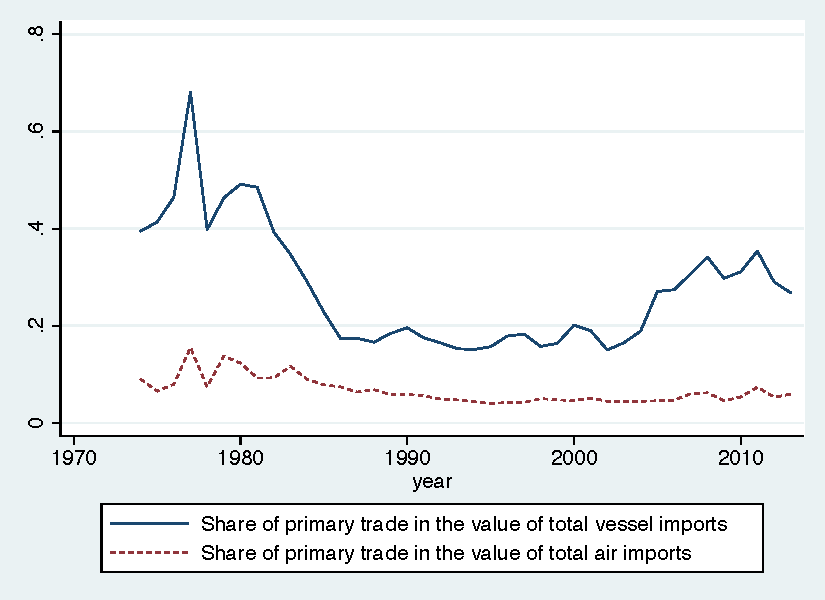
\includegraphics[height=4in]
{Share_of_primary.pdf}
\end{center}
\end{figure}

\textbf{A commenter. A mettre en Online Appendix?}






\subsection{Detailed Results \label{secoa:detailed}}
\setcounter{table}{0}
\renewcommand{\thetable}{B.\arabic{table}}


\subsubsection{3-Digits Level}

\subsubsection{4-Digits Level}




\end{document}





